\chapter{Software usage purpose }
\label{ch:purpose}
 

%
% Section: intro
%
\section{Introduction}
\label{sec:purpose:intro}

In scientific investigations broad range of software is being employed for various purposes. In terms of size, software ranges from simple script to extremely complex one with millions of lines of code. In terms task, a software can be used for execution of rudimentary tasks to computation of extremely complex ones. Typical examples of purpose of software use for scientific investigation are simulation, modeling, data analysis, etc. \citep{goble2014better}. \\


To be able to automatically identify, from context, for what purpose a software is used in a scientific paper, a classifier algorithm has to be trained on a manually annotated dateset that indicate software usage purpose. The \ac{SoMeSci} data set already has annotations about type of software, type of software mentions, etc. and only require extension with software purpose annotation so that it can be used for training a software usage purpose classifier. However, a comprehensive list of potential software usage purposes has to be identified before hand. To enumerate possible software purposes of usage, three things have been done in this thesis. These are:
analysis of literature,  software ontologies and Sci-Crunch repository. The process work flow is shown on the figure 3.1. as follows.  

\begin{figure}[htbp]
	\centering
	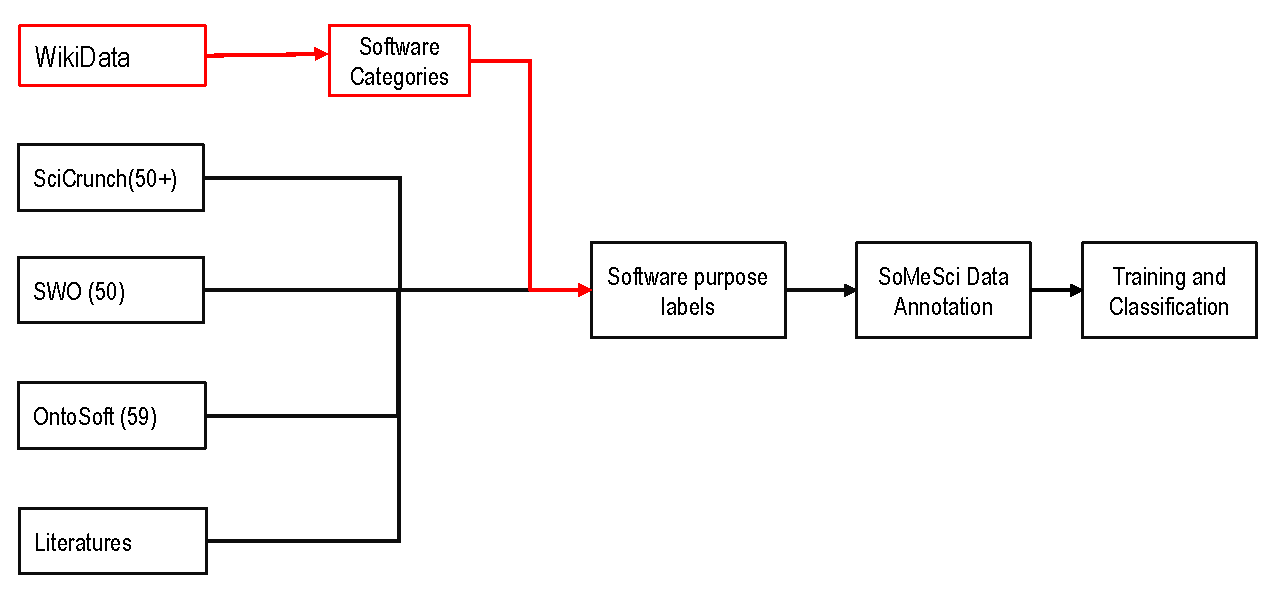
\includegraphics[width=1\textwidth]{4.graphics/figures/ch_3/softwarePurposeprocess}
	\caption{Workflow indicates a sequence of steps followed to extract classes of potential software usage purposes to label data set that will be used to train a classifier }
	\label{fig:chapter03:setup}
\end{figure}


After identifying a list of potential software usage purposes, the list has been consolidated further to narrow down the list to a more comprehensive list of software usage purposes for convenience during annotation of data set. \\

This section elaborates the analysis procedure of a list of resources mentioned above to identify possible software usage purposes.  
 

%-----------------------------
\section{Analysis of literature }
\label{sec:purpose:literatures}
%-----------------------------

In a research, scientists follow scientific method to discover knowledge. Typically, scientists begin with a question and attempt to answer questions through a research and propose hypothetical answers for their questions. Then, they test the proposed hypothesis by conducting various experiments. Although all scientists do not follow the exact same procedure, the over all idea remains the same {enwiki:1061107378- Scientific method}. This is where a software use comes into play, aid scientists during their experiment. \\

Therefore, the analysis of literature when looking for software usage purpose is aimed at answering, from a given context, \emph{“for what purpose scientists are using a software ?”} in their experiments.\\

Accordingly, some key words that reflect potential software usage purposes have been identified from the literature and listed on the following table:



%...

\begin{table}[h!]
	\begin{center}
		\caption{Key words that has been extracted from analysis of literature that potentially indicate purpose of software use.}
		\label{tab:table1}
		\begin{tabular}{|l|l|} % <-- Changed to S here.
			
			%\textbf{Value 1} & \textbf{Value 2} \\
			\hline
			- Comparison of experimental groups & -	Statistical analysis  \\
			- Quantification & - Data analysis \\
			- Measurements   & - Densitometric analysis \\
			- Analysis       & - Voxel-based Analysis  \\
			- Mapping        & - Cross-sectional ROI analysis \\
			- Correction of mapping  & - Gene analysis     \\
			- Generate scaffolds     & - Gene assembling \\
			- Generate trees         & - Construct contigs \\
			- Search sequences       & - Fill gaps \\
			- Map                    & - Generate assembly \\
			- Predict gene structure & - Calculate \\
			- Align gene             & - Draw heat map \\
			- Filter                 & - Validate \\
			- Evaluate               & - Annotation \\
			- Select                 & - Fit or train a model \\ 
			- Optimise               & - Sketch \\
			- Classify               & - Identify \\
			
			\hline
		\end{tabular}
	\end{center}
\end{table}

The list of key words in the above table is used to delineate possible software usage purposes, however, it is intractable to enumerate all possible software purposes by manually reading through unlimited number of publications. To augment results obtained from the analysis of literature, various software ontologies and repositories like, Sci-Crunch, have been analyzed as presented in the following section. 


%-----------------------------
\section{Analysis of software ontologies }
\label{sec:purpose:ontologies}
%-----------------------------

Ontologies are controlled vocabularies that provide formal naming and definition of properties and relation between concepts, entities, data etc.  Ontologies  are specialized  to a specific subject matter and every academic discipline creates ontologies to organize data into useful knowledge \citep{enwiki:1060388948}. \\

Effective knowledge representation begins with analysis of ontologies with in the domain of interest \citep{chandrasekaran1999ontologies}. Accordingly, analysis of software ontologies have been done to find out possible software usage purposes. The software ontologies, that has been analyzed on this project are: WikiData \footnote{https://wikidata.org/}, \ac{SWO} \footnote{https://www.ebi.ac.uk/ols/ontologies/swo}, and Ontosoft\footnote{https://www.ontosoft.org/}. 

 
%-----------------------------
\subsection{Wikidata}
\label{subsec:purpose:ontologies:Wikidata}
%-----------------------------

Wikidata is a multilingual knowledge graph that is curated collaboratively by a Wikimedia community and serves as a freely available common source of structured data for everyone \citep{enwiki:1060114687, enwiki:1060408581}. \\

Wikidata was created by Wikimedia foundation mainly to store meta data that can be used for other Wikimedia projects such as Wikipedia. Interestingly, wikidata is allowed to contain inconsistent and contradicting facts in order to embrace the diversity of knowledge about a given entity \citep{vrandevcic2012wikidata}. \\

Although wikidata has a tremendous amount of data in it, there was no information that would indicate software usage purposes, rather information about software categories was found. Therefore, an indirect approach has been taken to list down possible software purposes from software categories by assuming each software category has essentially a software purpose associated to it. \\

Wikidata has a bunch of tools like, SPARQL end point, query builder, data visualization tools, etc. Thus a SPARQL end point has been utilized  to query a list software and their potential categories in a format that supports network analysis, with edge and node. As a result, over 400 software categories have been found from the Query. The SPARQL query used to retrieve software categories have been listed under \emph{Appendix A}.\\

To find out potential relation between these categories and to select more general software categories, a network analysis has been done using Gephi software (version 0.9.2) \footnote{http://gephi.org/}. Using Gephi, clustering of related software categories and filtering has been made to identify a more generalized software categories. \\

\noindent The procedure for network analysis has been described as follows:

\begin{itemize}
	\itemsep1em
	\item First query result from the SPARQL terminal of wikidata has been downloaded in a csv file format. 
	\item Then, the csv file has been opened with Gephi software (version 0.9.2) as \emph{“undirected graph”}. This renders a network graph with overlapping nodes and edges. 
	\item To unravel the overlapping nodes for visibility, the lay-out of the graph is then changed to \emph{“Fruchterman Reingold”}. 
	\item To find out possible clusters from the network, from the list of statistical tools, \emph{“Modularity”} has been run. Then partition of nodes and edges has been done using \emph{“Modularity class”}. 
	\item Then to adjust size of nodes based on importance, node size ranking has been done with a \emph{“Degree”} parameter with \{minimum, maximum\} size of  \{20, 80\} respectively. 
	\item Then to select the most prominent nodes, among filter tool \emph{“Degree range”} filter has been used. The Degree range filter estimated prominence of the nodes between values of \{1, 60\} where the maximum value indicates the most prominent node. 
\end{itemize}

\begin{figure}[h]
	\myfloatalign
	\subfloat[Degree \{1-60\}]{
		\label{fig:chapter03:subfloat:grafik1}
		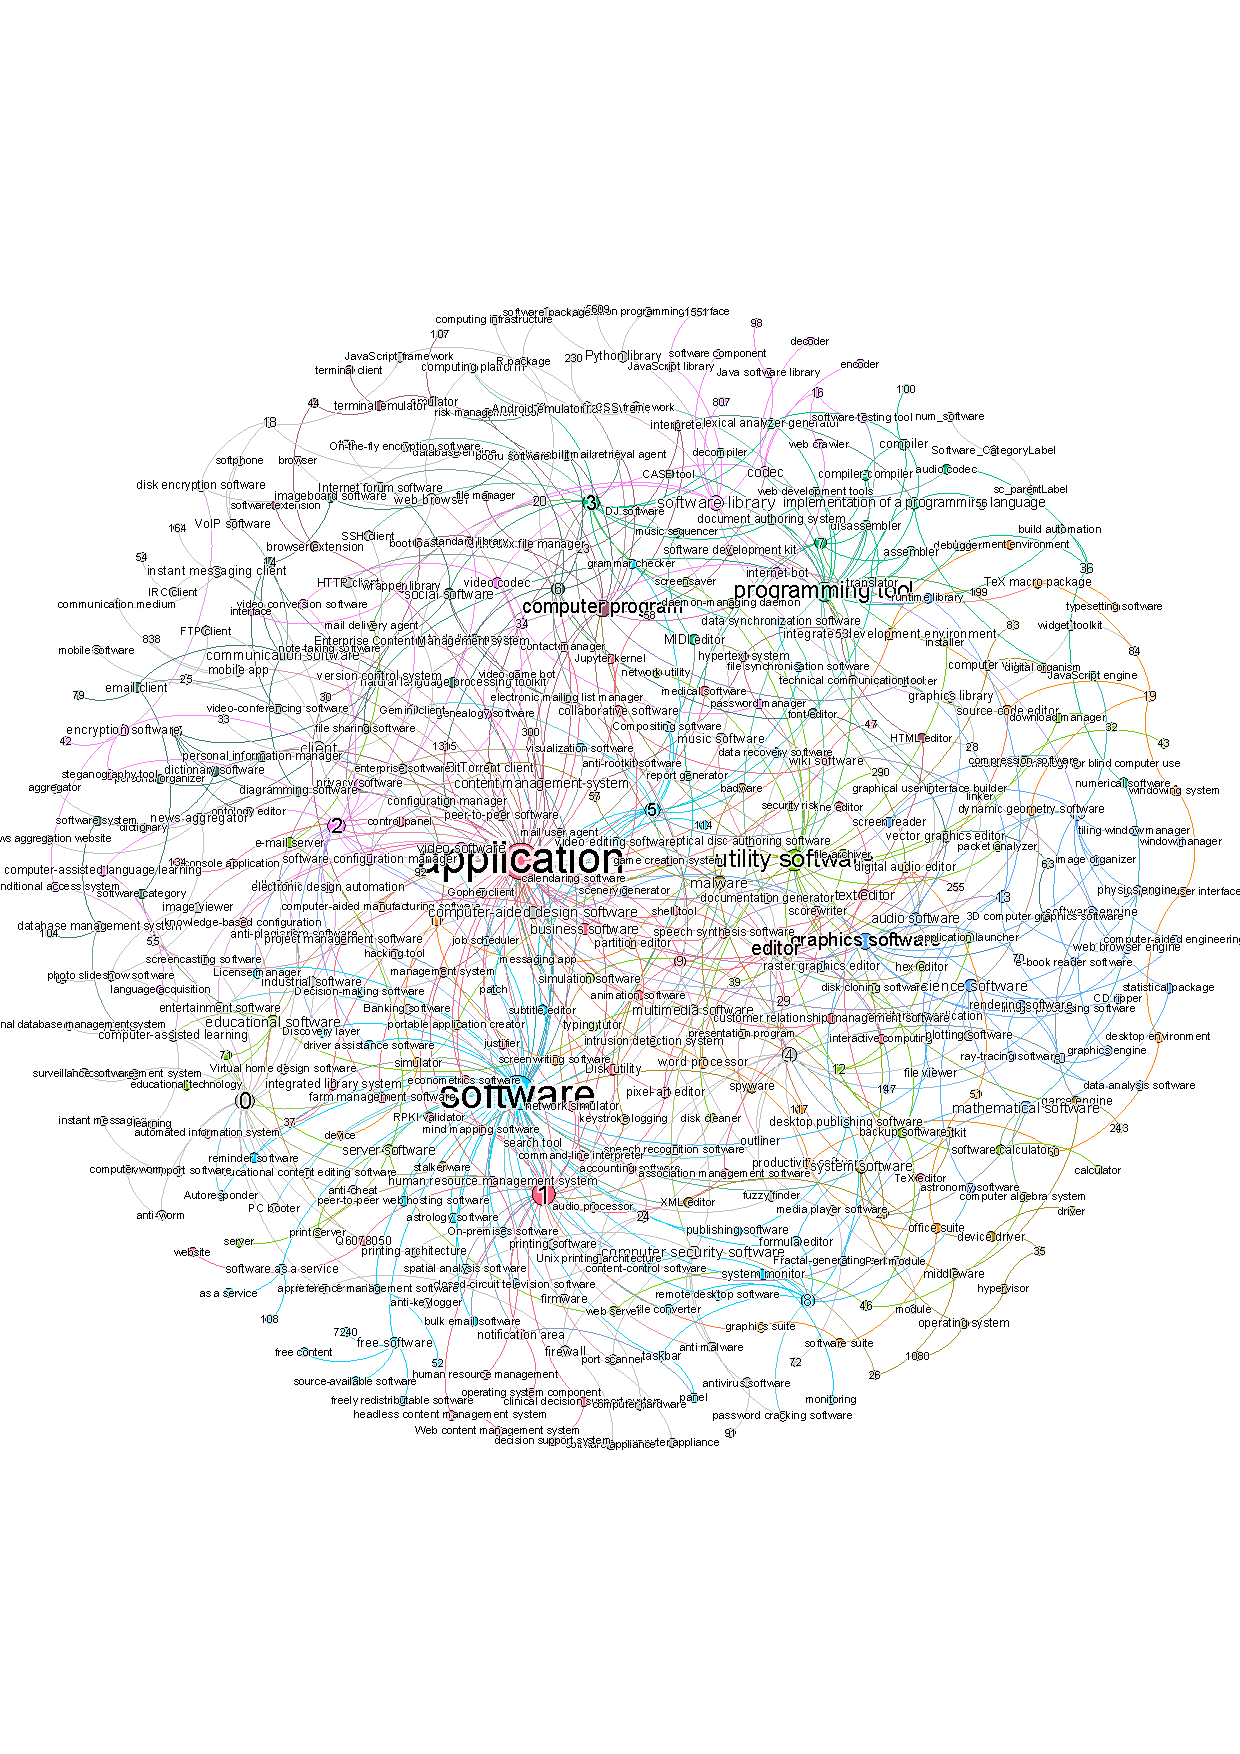
\includegraphics[width=.25\linewidth]{4.graphics/figures/ch_3/Network1}
	} \quad
	\subfloat[Degree \{3-60\}.] {
		\label{fig:chapter03:subfloat:grafik2}
		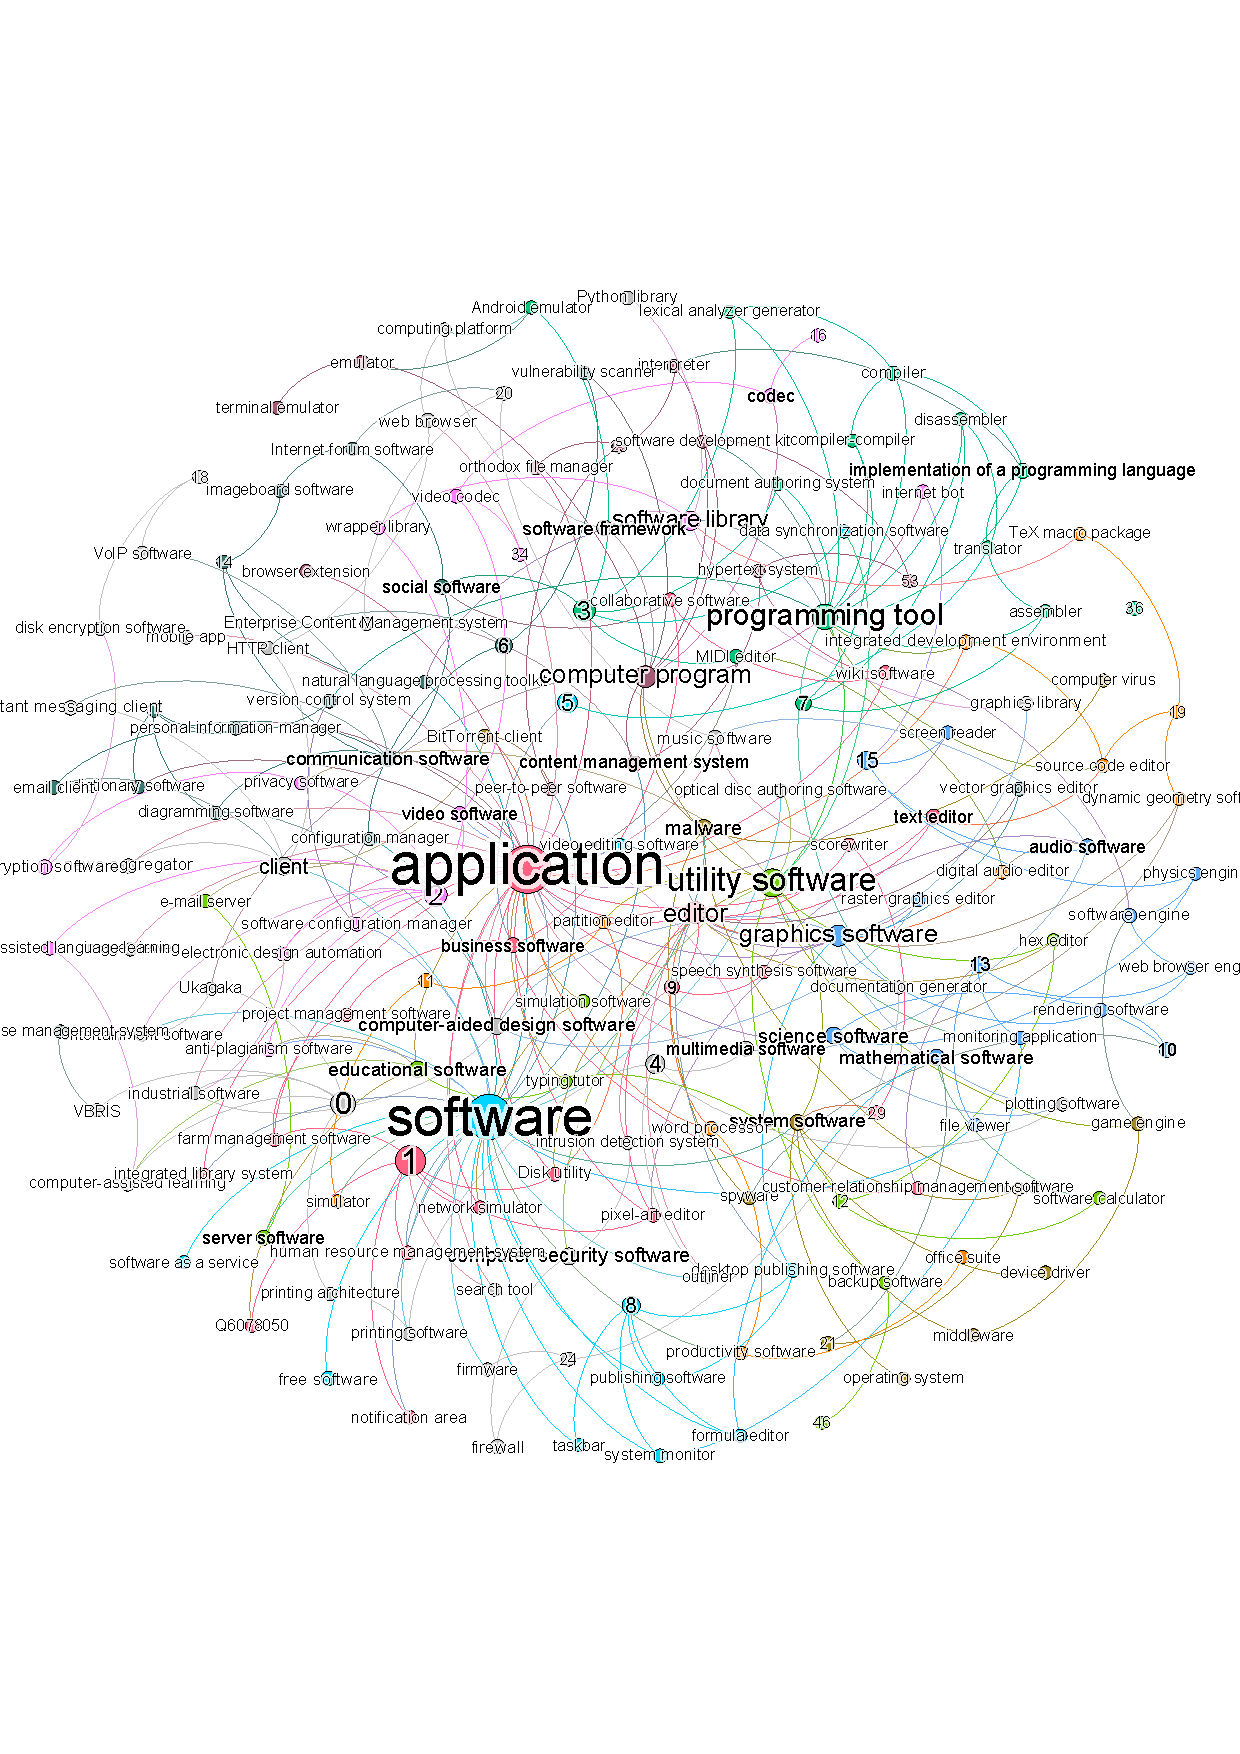
\includegraphics[width=.25\linewidth]{4.graphics/figures/ch_3/Network2}
	} \\
	\subfloat[Degree \{5-60\}]{
		\label{fig:chapter03:subfloat:grafik3}
		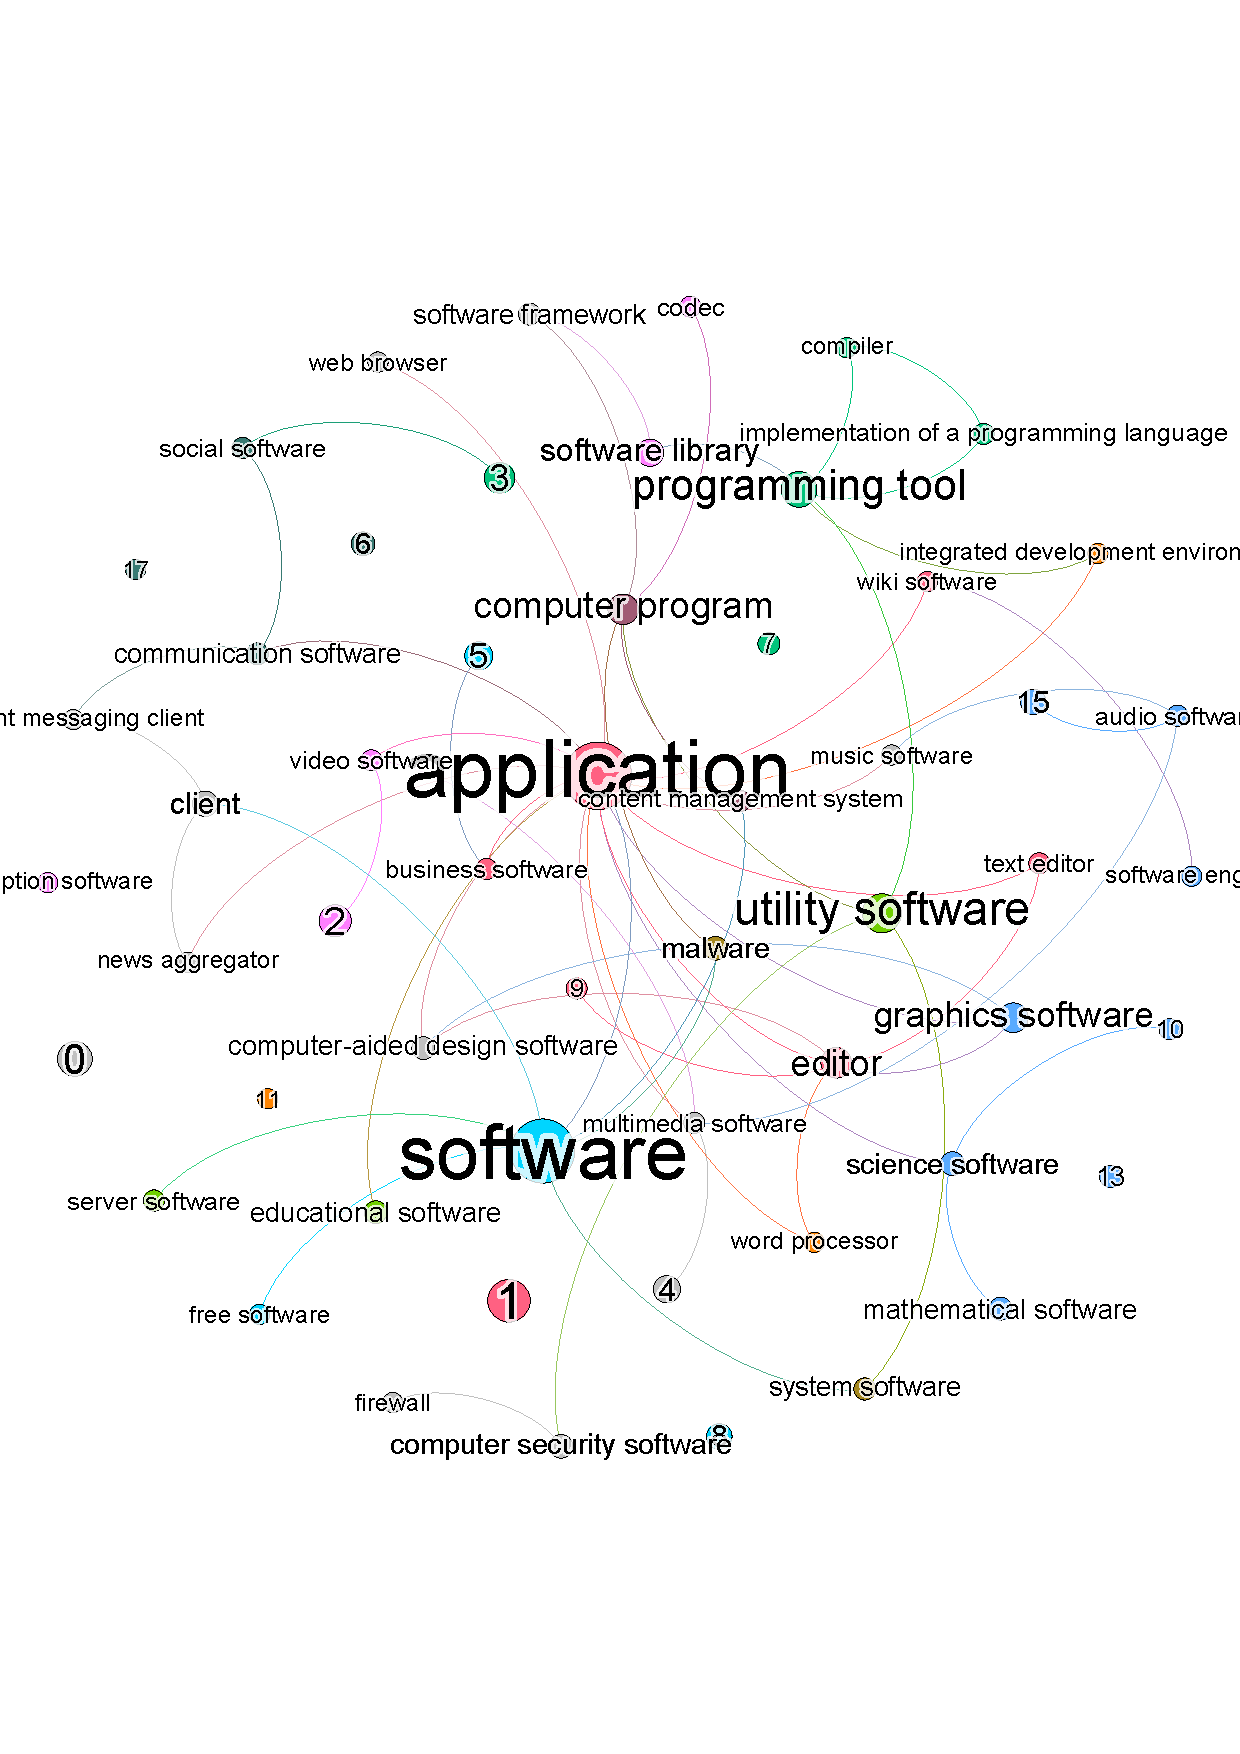
\includegraphics[width=.25\linewidth]{4.graphics/figures/ch_3/Network3}
	}
	\subfloat[Degree \{7-60\}]{
	\label{fig:chapter03:subfloat:grafik4}
	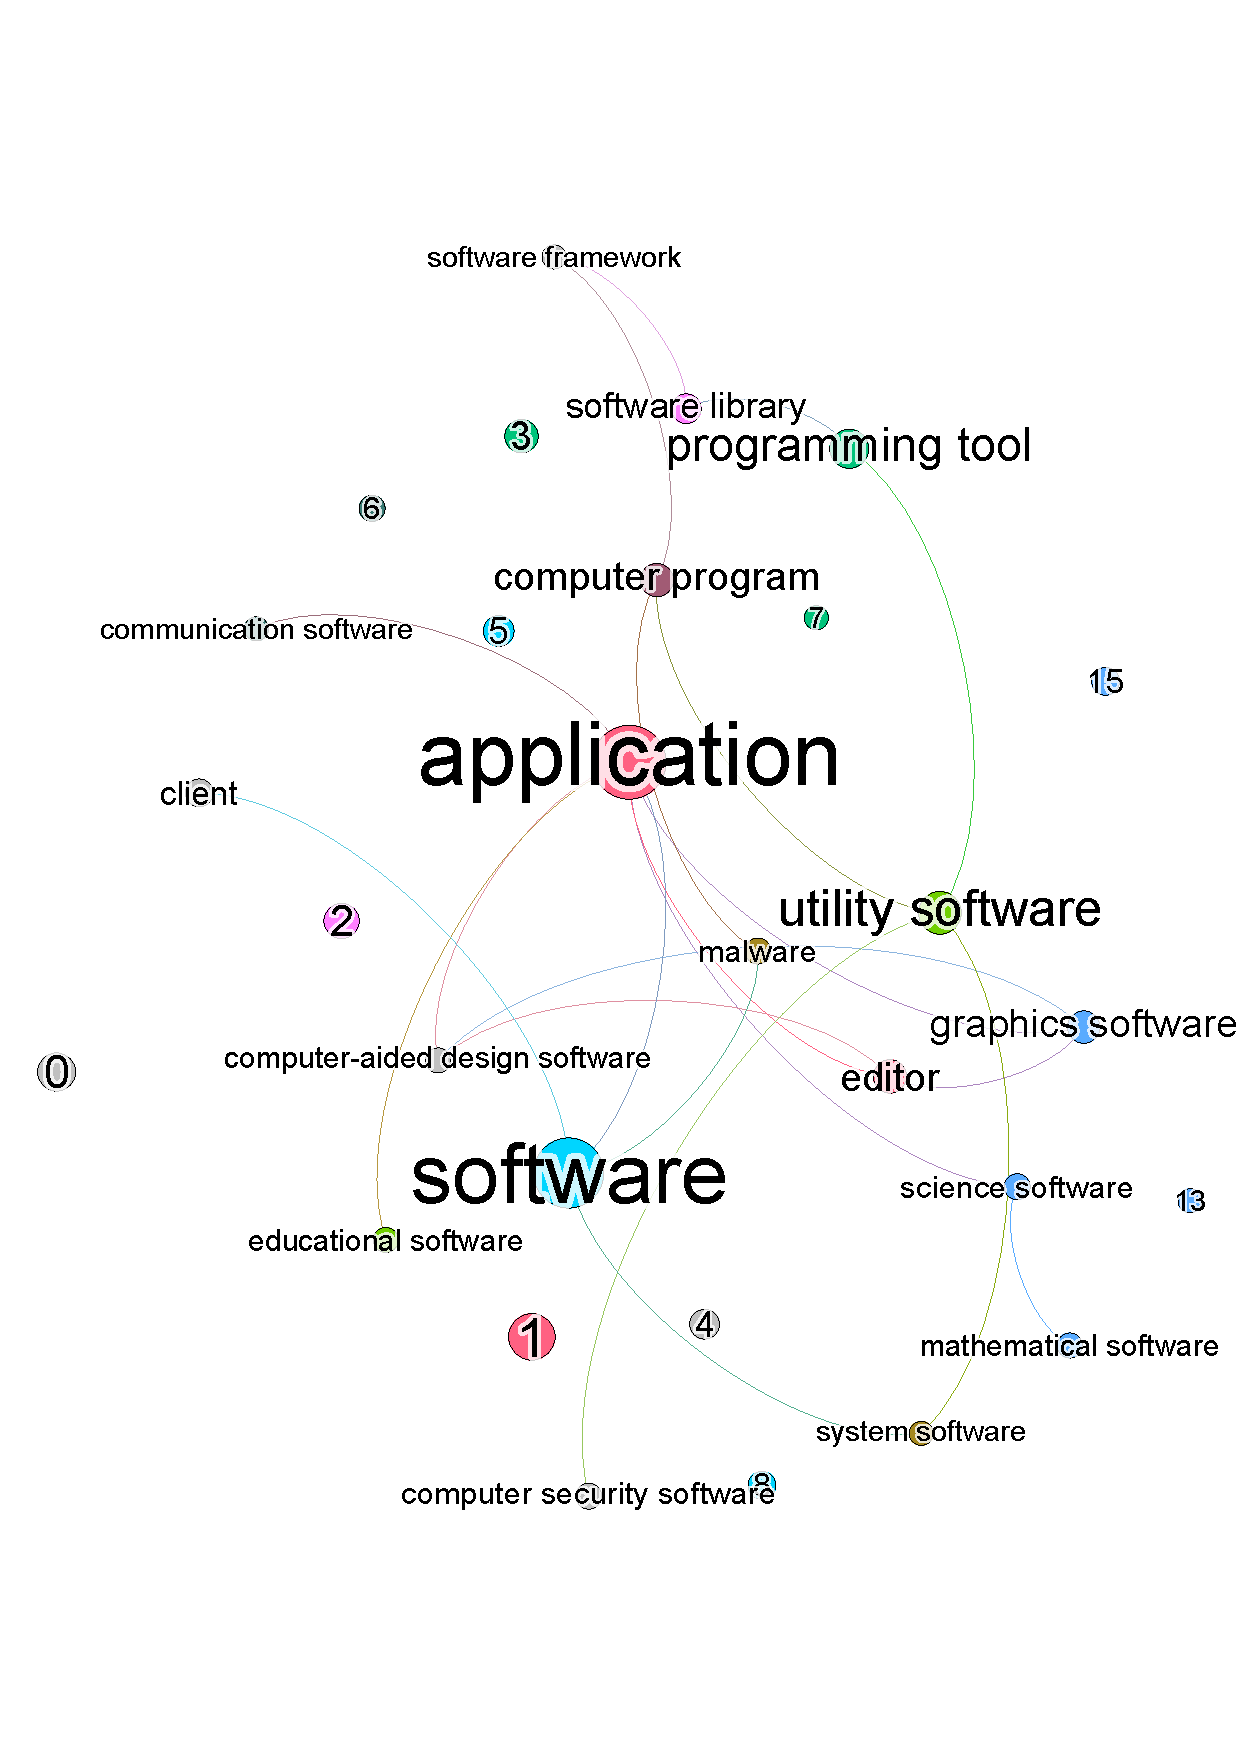
\includegraphics[width=.25\linewidth]{4.graphics/figures/ch_3/Network4}
	}\\
	\caption[Subfloat - Figure]{The result of network analysis from Gephi software - indicates the relation between each software category. The Degree filter with a range of 1 to 60 indicates prominence of a node in the network. Large value correspondences to a more general parent node (more general software category).}

\end{figure}


\noindent According to the network analysis, the major types of software categories identified are listed on the table below.
\\
\begin{table}[h!]
	\begin{center}
		\caption{Major software categories identified with network analysis of data retrieved from Wikidata with SPARQL Query.}
		\label{tab:table1}
		\begin{tabular}{|l|l|} % <-- Changed to S here.
			
			%\textbf{Value 1} & \textbf{Value 2} \\
			\hline
			- Application softwares & -	Utility software  \\
			- Computer security software & - System software \\
			- Measurements   & - Densitometric analysis \\
			- Client       & - Programming tool   \\
			- Software Library        & - Software framework  \\
			- Editor  & - Science software     \\
			- Graphics software     & - Computer aided design software \\
			- Mathematical software          & - Communication software \\
			\hline
		\end{tabular}
	\end{center}
\end{table}

According to a manual analysis of wikidata, software categories listed  in table above are related to each other as well. Mathematical software, for instance, is subclass of science software and science software is subclass of application software. \\

By further analyzing the relation between the software categories in the table above, overall the three main types of software categories identified are:  Application software, System software and Software Component. A simplified version of  hierarchical relation between these categories is depicted on figure 3.3. 

\begin{figure}[htbp]
	\centering
	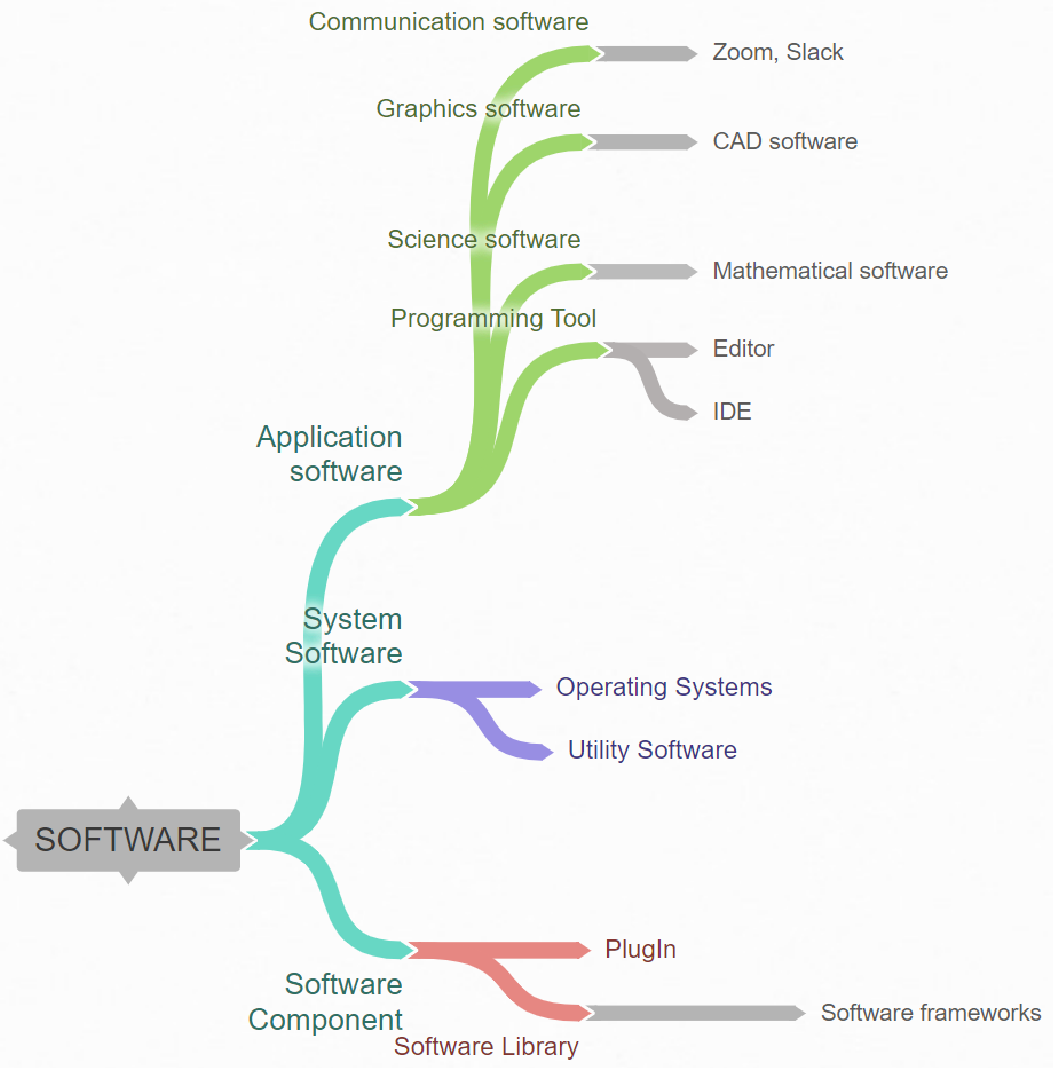
\includegraphics[width=.73\textwidth]{4.graphics/figures/ch_3/chart}
	\caption{Relation between the three main software categories identified from WikiData.}
	\label{fig:chapter03:setup}
\end{figure}


%-----------------------------
\subsection{The software ontology (SWO)}
\label{subsec:purpose:ontologies:SWO}
%-----------------------------

The \ac{SWO}), particularly describes software used, for preparation and maintenance of data, within fields of computational biology and bio-informatics.  The \ac{SWO} was primarily developed to improve reproducibility by providing detailed description about software used for biomedical investigations \citep{malone2014software}. \\

\ac{SWO} was found on ontology search \ac{OLS} website \footnote{https://www.ebi.ac.uk/ols/ontologies/swo} and was examined for possible software purposes. Unlike wikidata, a list of possible software purpose were found directly in “browse terms” section of the SWO website.  \\

To navigate to the list of key words that suggest potential software purpose one can follow the following steps: “Browse terms”> “entity“>”occurrent”> “planned” >”planned process”.  The software usage purpose in the SWO has been presented in to two main groups as “data transformation” and “data visualization”.  Under data transformation, 40 sub-types of potential software purposes are listed as shown on figure below. \\


\begin{figure}[htbp]
	\centering
	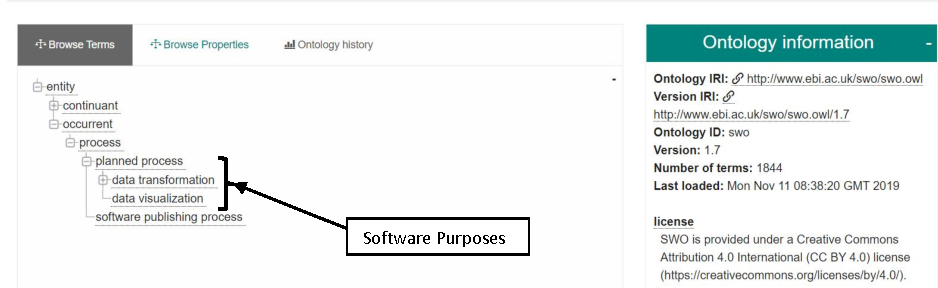
\includegraphics[width=.99\textwidth]{4.graphics/figures/ch_3/SWO2}
	\caption{List of key words that indicate software usage purposes on the SWO Ontology website. Inside the data transformation section, there are 40 software usage purposes}
	\label{fig:chapter03:setup}
\end{figure}

Some examples of software usage purposes retrieved from SWO are shown on the table 3.3 below.

\begin{table}[h!]
	\begin{center}
		\caption{Few examples of software usage purposes extracted from the SWO Ontology.}
		\label{tab:table1}
		\begin{tabular}{|l|l|} % <-- Changed to S here.
			
			%\textbf{Value 1} & \textbf{Value 2} \\
			\hline
			- Data transformation & - Calculation  \\
			- Genome annotation   & - citation management  \\
			- Class discovery     & - dataset comparison   \\
			- Annotation          & - Analysis \\
			- Text editing        & - Data visualization  \\
			- Modeling           & - File rendering   \\
			- Curve fitting       & - Matrix manipulation  \\
			- Simulation          & - Data mining task   \\
			- Query and retrieval & - Clustering task \\
			- Distance calculation & - Image compression \\
			- Molecular sequence analysis & - Data Normalization \\
			- Decision tree induction & - Descriptive statistical analysis \\
			
			\hline
		\end{tabular}
	\end{center}
\end{table}


%-----------------------------
\subsection{OntoSoft}
\label{subsec:purpose:ontologies:OntoSoft}
%-----------------------------
Onosoft is a software registry framework that stores important metadata about software to foster reuse and sharing of software among scientific community. The ontology provides descriptions about a software that would help scientists to identify, understand, execute, and do research with a software. Moreover, it helps scientists get information about update and support for the software. \\

These descriptions are visualized in a 6 dimensional pie-chart, with each slice indicating the completeness of the description. Particularly, Ontosoft focuses on the geo-science because software resources are not being shared adequately in that field \citep{gil2015ontosoft}.

The type of information provided in each dimension of description entries are  summarized in the table below:



\begin{table}
	\caption{The six dimensions of information description in the Ontosoft software ontology}
	\begin{tabularx}{\textwidth}
		{|>{\setlength\hsize{.6\hsize}\setlength\linewidth{\hsize}}X|>{\setlength\hsize{1.4\hsize}\setlength\linewidth{\hsize}}X|}
		
		\hline
		DIMENSION & DESCRIPTION  \\
		\hline
		Identify   &
		-  Name/abbreviation of software,  etc.\\
		\hline
		Understand & -  domain specific key words ,  software creator, ...etc.\\
		\hline
		Execute    & -	URL, license, system requirements …etc.  \\
		\hline
		Do Research & -	file formats, preferred citation information, …etc.   \\
		\hline
		Get support & -	Contact details, possible support included, etc.  \\
		\hline
		Update      & - Version, developer community, maintenance, etc.  \\
		\hline
	
		
	\end{tabularx}
\end{table}

From the set of information provided among the 6 dimensions of the Ontosoft, particularly the “understand” dimension has nearly 400 domain specific key words that would potentially indicate software usage purposes. Therefore, those domain specific key words has been retrieved, analyzed and condensed into a more general software purposes. \\

Sample list of domain specific key-words that would potentially indicate a software usage purpose is listed on the following table. 

\begin{table}[h!]
	\begin{center}
		\caption{Few examples of key-words extracted from Ontosoft ontology that indicate potential use of software.}
		\label{tab:table1}
		\begin{tabular}{|l|l|} % <-- Changed to S here.
			
			%\textbf{Value 1} & \textbf{Value 2} \\
			\hline
			\multicolumn{2}{|c|}{Domain specific Key words }\\
			\hline
			-	Data manipulation & -	Numerical model \\
			-	Data Mining       & -	Numerical simulation \\
			-	Image processing  & -   Thermal model \\
			-	Machine learning  & -   Integrated modeling \\
			-	Simulation- optimization & - Interactive visualization \\
			-	Network analysis & - Wind wave estimation \\
			- 3D printing         & - data integration \\
			- geospatial data conversion & - Image Processing \\
			- Computer Vision & - Machine Learning \\
			- Interactive Visualization & - Numerical simulation \\
			- network analysis & - Performance Evaluation \\
			- Visualization & -  Wind wave estimation \\
			\hline
		\end{tabular}
	\end{center}
\end{table}

%-----------------------------
\section{Analysis of Sci-crunch repository }
\label{sec:purpose:Sci}
%-----------------------------

The other resource analyzed in addition to software ontologies is to list down software usage purposes is Sci-crunch \footnote{https://scicrunch.org/} repository. Sci-crunch is a data portal that searches through hundreds of community databases, aggregates information resources to create a large collection of data and tools available for access at a single spot \citep{grethe2016scicrunch}. \\

To identify possible software usage purposes, the Sci-crunch repository has been analyzed as follows. On the registry section of the sci-crunch home page, there is a pie chart indicating different types of resources. A software resource, with  7,155 different types of software resources has been selected from the pie chart. From there, top 200 types of software resources have been identified using the site’s built in word-cloud generator. \\
 

\begin{figure}[htbp]
	\centering
	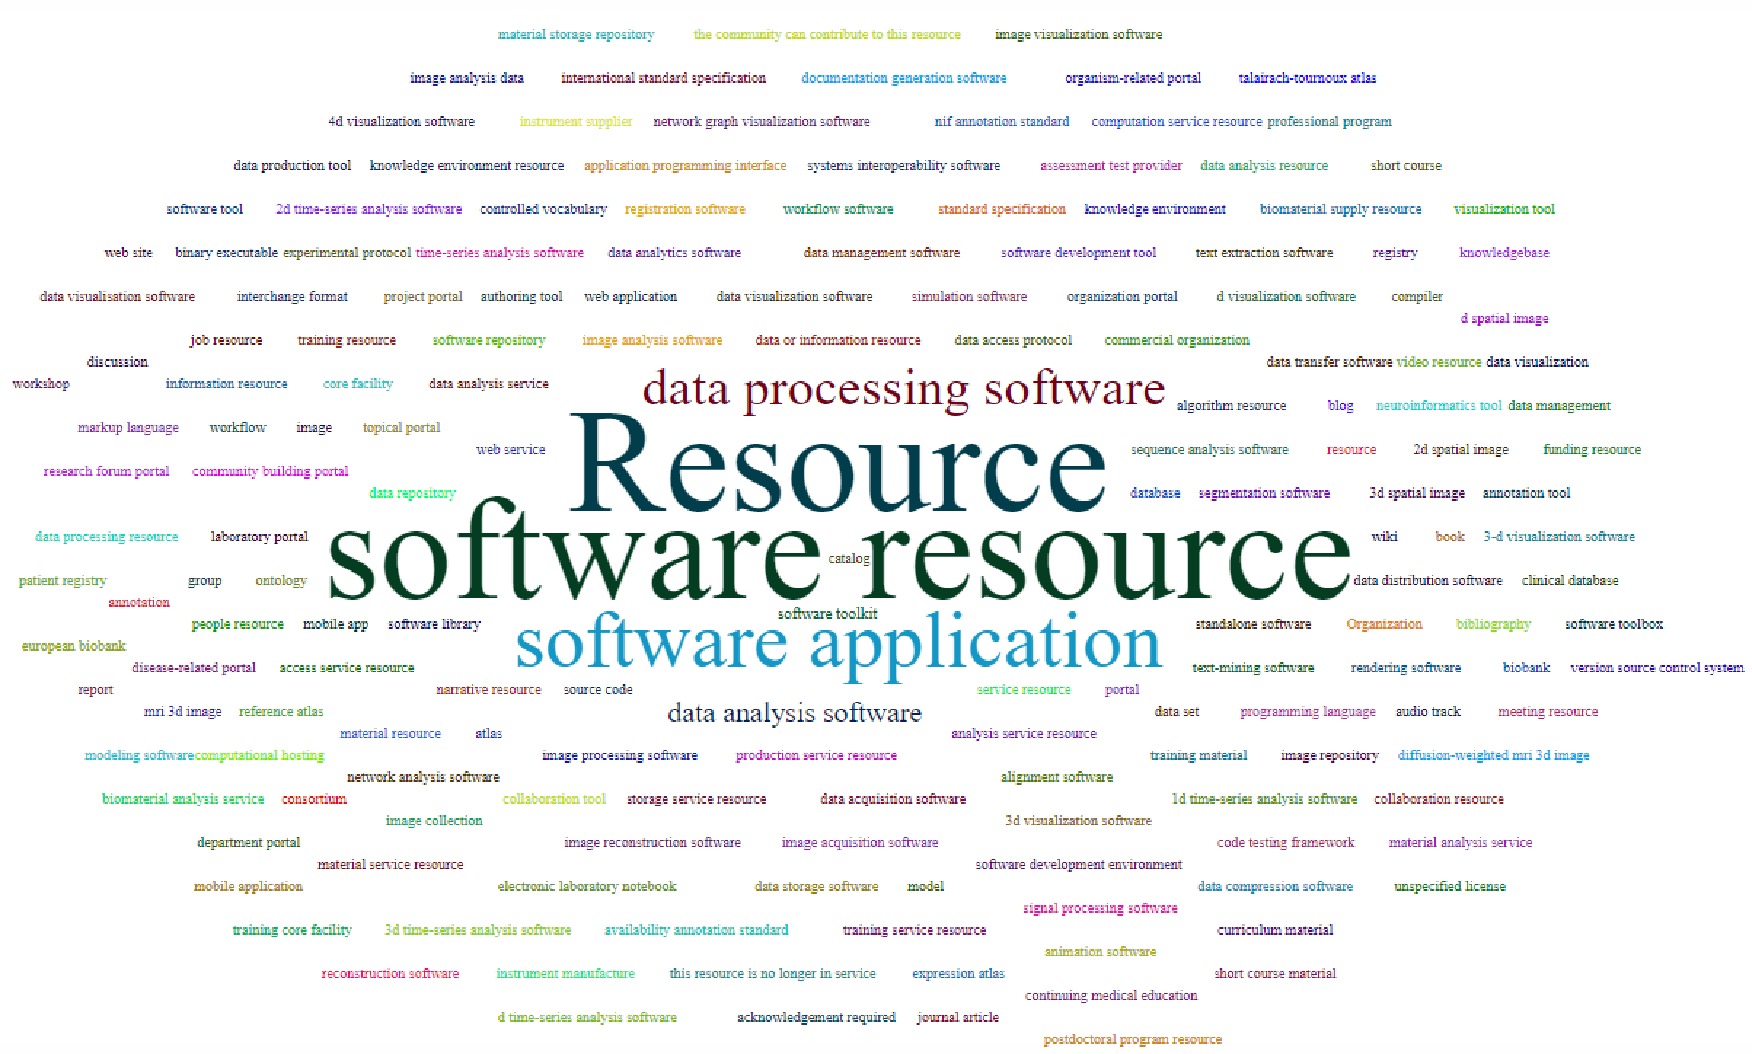
\includegraphics[width=.75\textwidth]{4.graphics/figures/ch_3/cloud}
	\caption{Word cloud retrieved from Sci-crunch repository indicating 200 different types of software that  indicate potential purpose of software usage}
	\label{fig:chapter03:setup}
\end{figure}

After a manual analysis of the 200 of software types, generated from the word cloud, important software types that indicate possible software usage purpose has been identified. Sample of software types and their corresponding usage purpose is summarized on table 3.4.

\begin{table}[h!]
	\begin{center}
		\caption{software types and potential purpose.}
		\label{tab:table1}
		\begin{tabular}{|l|l|} % <-- Changed to S here.
			\hline
			\textbf{Software Type} & \textbf{Purpose} \\
			\hline
			- Data acquisition software, Image acquisition software  & - Data collection, Recording  \\
			\hline
			- Data / Image  / Sequence  / Network  Analysis software  & - Data Analysis  \\
			\hline
			- Text mining software  & - Data Analysis  \\
			\hline
			- Signal processing software  & - Data Analysis  \\
			\hline
			- Data / 3D Visualization software & - Data Visualization  \\
			\hline
			- Simulation software  & - Simulation  \\
			\hline
			- Alignment software  & - Data pre/post-processing \\
			\hline
			- Rendering software  & - Modeling  \\
			\hline
			-	Code testing framework   & - programming  \\
			\hline
		\end{tabular}
	\end{center}
\end{table}


%-----------------------------
\section{Types of software usage purposes }
\label{sec:purpose:Types}
%-----------------------------

Based on a through analysis of scientific literature in \ac{SoMeSci} dataset, software ontologies and the sci-crunch repository, overall 8 main types of software usage purpose have been identified. These are: 

\begin{itemize}
	\itemsep0em
	\item Data collection / recording  
	\item Data pre-processing
	\item Analysis 
	\item Visualization
	\item Simulation
	\item stimulation 
	\item Modelling
	\item Programming
\end{itemize}

To establish a clear boundary and avoid ambiguity during the annotation process of software usage statements, in \ac{SoMeSci} data set, each software usage purpose has been clearly defined based on literature in the next section as follows. 



\subsection{Data collection}
\label{sec:purpose:Types:datacollection}


According to Wikipedia, data collection is a process of collecting, recording or measuring information on targeted variables which enables answering of questions. Regardless of the type of data, quantitative or qualitative, data collection is one of the most important steps in a scientific investigation \citep{enwiki:1049936190}. \\

Scientists collect data for their research using various data collection software tools and gadgets. In one research, for instance, scientists used an Actigraph Reader Interface Unit (RIU-41A) with its software to measure the level of activity of more than 5000 children of age 12 to characterize the relation between physical activity and obesity \citep{ness2007objectively, enwiki:1046731490}. \\

Often times data pre-processing involves several steps such as data cleaning, integration, transformation, reduction, etc. \citep{malley2016data}. Data cleaning, for instance, involves dropping of data, replacing, or imputation of missing values in order to improve performance of algorithms and reliability of analysis results, especially in data mining applications \citep{enwiki:1051181443, enwiki:1056727993}. In a scientific investigation, scientists usually carry out data pre-processing using a custom script or using an existing application software or programming library. \\

\subsection{Data Analysis}
\label{sec:purpose:Types:Analysis}

Data analysis refers to processing, transforming, modeling, etc. of data with a goal of discovering a new insight that would support conclusions or decision making. Data analysis involves diverse techniques with different names in various domains. \citep{enwiki:1061024140}. In their research, scientists employ various software to carry out various tasks of data analysis such as  curve fitting, spectral smoothing using a software \citep{proctor1982data}. 

\subsection{Data visualization}
\label{sec:purpose:Types:visualization}

Data visualization refers to techniques that are used to communicate data or information effectively in the form of visual objects such as points, lines, bars, etc. in a graphic representation \citep{enwiki:1059912747}.  

\subsection{Simulation}
\label{sec:purpose:Types:Simulation}

Computer simulations mimic operation of real-world process or system using models that represent key-behaviors of the system. By varying variables of the simulation, predictions about behavior of systems can be made. Simulations have a wide range of application in scientific modeling of natural systems in physics, chemistry and biology \citep{enwiki:1061669086}. Simulations are run to improve understanding of a problem  \citep{segal2008developing}.


\subsection{Stimulation}
\label{sec:purpose:Types:Stimulation}

Stimulation is the act of evoking the development of involuntary activity or response. Living organisms have sensory receptors that generate impulses that travel through nerve to the brain upon a reception of excitation by means of various agents, energy, collectively known as stimuli. Examples of sensory receptors in the human body are photo-receptors in the retina, touch receptors on the skin, chemical receptors in mouth, etc. \citep{enwiki:976395276}. 
In the scientific investigations, scientists use various mechanisms to provide a stimulation to their research object. One of the ways to provide stimulation is using a software. In neurological research, for example, scientists use various brain stimulation techniques and software to study neurological disorders.  Deep Brain Stimulation (DBS), for instance, is one of brain stimulation techniques used to treat diseases like Parkinson’s, essential tremor, dystonia etc. \citep{schermer2011ethical}.




\subsection{Modeling}
\label{sec:purpose:Types:Modelling}

Modeling refers to scientific activities that aim to facilitate understanding of a particular feature or phenomena in the world. It is a process of identifying and selecting relevant aspects of a situation or phenomenon under consideration. Different types of models with more specific aim exist.  For instance, conceptual modeling provide better understanding, mathematical models help to quantify, computational models are used for simulation, etc. \citep{enwiki:1051627717}.\\

Modeling is a broad term that refers to a wide range of activities. It might refer to 3D modeling and graphical representation of a real world physical objects like vehicles, buildings, …etc.  using Computer Aided Design (CAD) software. For instance, some scientists use graphical modeling software, for instance for digitally documenting historical sites such as castles \citep{el2007detailed}. On the other hand modeling can also refer to mathematical representation of a non physical abstract entity. In one research paper, for instance, the researchers were trying to model the occurrence of letters and word’s initials mathematically \citep{pande2010mathematical}. 

Regardless of the wide meaning and techniques of modeling, inherently all models serve to represent an object or a system to facilitate the representation, or understanding of particular feature or phenomena \citep{enwiki:1058944086, enwiki:1051627717}.  


\subsection{Programing}
\label{sec:purpose:Types:Programing}
Programming refers to the process of designing and building executable computer programs that performs a specific task. Computer programs are written in a human readable format mainly to automate execution of complex tasks and for solving problems \citep{enwiki:1062649903}. \\
\\

Summary of software usage purposes and corresponding examples are summarized in the table below:

\begin{table}
	\caption{Brief summary of software usage purposes and examples.}
	\begin{tabularx}{\textwidth}
		{|>{\setlength\hsize{.6\hsize}\setlength\linewidth{\hsize}}X|>{\setlength\hsize{1.4\hsize}\setlength\linewidth{\hsize}}X|}
		
		\hline
		USAGE PURPOSE & Examples  \\
		\hline
		1. DATA COLLECTION    &
		\begin{itemize}
			\itemsep0em 
			\item Surveying, Data acquisition, Data recording, Text extraction, Measurement, Constructing an artificial data set, Importing a file or data of specific format into a software, ... etc.    
		\end{itemize} \\
		\hline
		2. DATA Pre-processing    &
		\begin{itemize}
			\itemsep0em
			\item Data cleaning, Data normalization,  Data encoding, Data reduction, Text editing, Error correction, Data type conversion , Missing data handling, Data transformation, Tabulating, merging data, File formatting, Aligning gene, ... etc.  
		\end{itemize} \\
		\hline
			3. ANALYSIS    &
		\begin{itemize}
			\itemsep0em
			\item Data manipulation, Tabulating, merging data, Testing hypothesis, Data mining,  clustering, Prediction, prediction, quantification,calculation, computation, comparing, testing, searching, assessing,  evaluating , ...etc.
			
		\end{itemize} \\
		\hline
		
		4. VISUALIZATION    &
		\begin{itemize}
			\itemsep0em
			\item Creating figures, Plotting, Graph/Figure generation, ... etc.		
		\end{itemize} \\
		\hline
		
		5. SIMULATION    &
		\begin{itemize}
			\itemsep0em
			\item Flight/ Event/Numerical/ simulation,  Flood dynamics simulation,  vehicle schedule simulation, etc. 
					
		\end{itemize} \\
		\hline
		
		6. STIMULATION    &
		\begin{itemize}
			\itemsep0em
			\item Stimulate behavior 
		\end{itemize} \\
		\hline
		7. MODELING    &
		\begin{itemize}
			\itemsep0em
			\item Scientific/Mathematical/ modeling,  Machine learning / Model fitting, Predicting a behavior, Estimating, Inference, ... etc. 
		\end{itemize} \\
		\hline
		
			8. PROGRAMMING    &
		\begin{itemize}
			\itemsep0em
			\item Programming, implementing, ...etc. 
		\end{itemize} \\
		\hline

	\end{tabularx}
\end{table}







